\documentclass[11pt]{article}
\usepackage[T1]{fontenc}
\usepackage[utf8]{inputenc}
\usepackage{lmodern,amsmath,amssymb,graphicx,geometry,microtype,setspace,booktabs,caption}
\usepackage[hidelinks]{hyperref}
\geometry{letterpaper,margin=1in}
\setlength{\parindent}{0pt}
\setlength{\parskip}{0.55em}
\setlength{\emergencystretch}{2em}
\captionsetup{labelfont=bf,font=small}
\renewcommand{\refname}{References}

\pagestyle{empty}
\renewcommand{\thefigure}{S\arabic{figure}}
\setcounter{figure}{2}

\begin{document}
\begin{figure}[!ht]\centering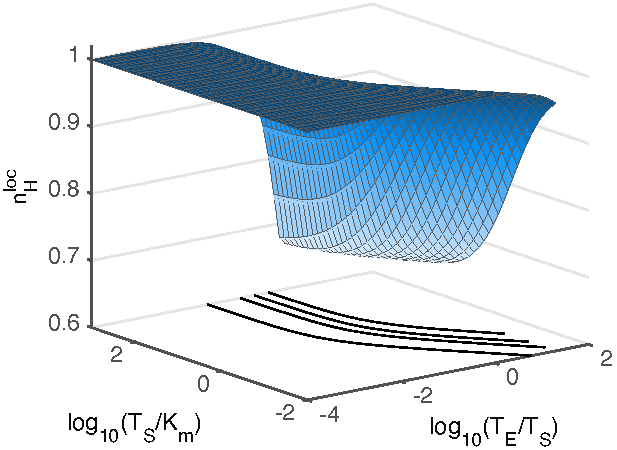
\includegraphics[width=\textwidth,height=0.65\textheight,keepaspectratio]{figure_inputs/FigS3_concentrations.pdf}\begin{singlespace}\caption{Concentration dependence of a total-target readout in a specified independent-site model. The plotted coefficient is the local negative logit slope with respect to free effector, evaluated where total modified fraction equals one-half. Parameters are $n=3$, $A=\widehat K=1$, $\widehat B=\widehat G=0.4$, and $K_m=1/(n\widehat B)$. Over the grid with $T_E/T_S\le0.01$, the coefficient lies between 0.99745 and approximately one. The result is a concentration-dependent total-response example; the exact free-target invariant concerns a different observable.}\end{singlespace}\end{figure}
\end{document}
